\documentclass{article}

\usepackage{microtype}
\usepackage{graphicx}
\usepackage{subcaption}
\usepackage{booktabs}
\usepackage{tikz}
\usetikzlibrary{positioning,arrows.meta}

% \usepackage[nohyperref]{icml2026}
\usepackage{hyperref}

\newcommand{\theHalgorithm}{\arabic{algorithm}}

\usepackage{icml2026}
% \usepackage[preprint]{icml2026}
% \usepackage[accepted]{icml2026}

\usepackage{amsmath}
\usepackage{amssymb}
\usepackage{mathtools}
\usepackage{amsthm}

\usepackage[capitalize,noabbrev]{cleveref}

\theoremstyle{plain}
\newtheorem{theorem}{Theorem}[section]
\newtheorem{proposition}[theorem]{Proposition}
\newtheorem{lemma}[theorem]{Lemma}
\newtheorem{corollary}[theorem]{Corollary}
\theoremstyle{definition}
\newtheorem{definition}[theorem]{Definition}
\newtheorem{assumption}[theorem]{Assumption}
\theoremstyle{remark}
\newtheorem{remark}[theorem]{Remark}

%\usepackage[disable,textsize=tiny]{todonotes}
\usepackage[textsize=tiny]{todonotes}

\usepackage{lipsum}
\usepackage{xcolor}
\let\oldlipsum\lipsum
\renewcommand{\lipsum}[1][1-7]{{\color{lightgray}\oldlipsum[#1]}}

\begin{document}

\twocolumn[
  \icmltitle{Speedrunning Tabular Foundation Models Pretraining}

  \icmlsetsymbol{equal}{*}

  \begin{icmlauthorlist}
    \icmlauthor{Salih Bora Öztürk}{ufr}
    \icmlauthor{Alexander Pfefferle}{ellis,ufr}
    \icmlauthor{Frank Hutter}{prior,ellis,ufr}
  \end{icmlauthorlist}

  \icmlaffiliation{ufr}{Department of Computer Science, University of Freiburg, Freiburg im Breisgau, Germany}
  \icmlaffiliation{ellis}{ELLIS Institute Tübingen, Tübingen, Germany}
  \icmlaffiliation{prior}{Prior Labs, Freiburg im Breisgau, Germany}

  \icmlcorrespondingauthor{Salih Bora Öztürk}{oeztuers@cs.uni-freiburg.de}

  \icmlkeywords{Machine Learning, Tabular Data, TabPFN, Foundation Models for Structured Data Workshop, ICML}

  \vskip 0.3in
]

\printAffiliationsAndNotice{}

\begin{abstract}
  \todo[inline]{single paragraph, ideally between 4--6 sentences, written at the end as the last thing}
  \lipsum[1]
\end{abstract}

\section{Introduction}

Structured data in tables is the bedrock of decision making~\citep{borisov2024dnntabular,vanbreugel2024position}.
Tabular foundation models (TFMs) are fundamentally changing the field, much as LLMs did for text~\citep{hollmann2023tabpfn,hollmann2025tabpfnv2,qu2025tabicl,qu2026tabiclv2,ma2025tabdpt,zhang2025limix}.
However, pretraining foundation models is computationally expensive, taking hours to days even at small scale and slowing research iteration.
Considerable work has tackled the problem of speeding up LLM pretraining~\citep{moddednanogpt,geiping2023cramming,deepseekv3,parametergolf2026}, but to our knowledge no equivalent effort exists for TFMs.
We close this gap with an open speedrun competition built around nanoTabPFN~\citep{pfefferle2025nanotabpfn}, empirically testing which techniques transfer.
Our best record reduces pretraining (todo:smth like baseline needed) from 74.32 to \textcolor{red}{XX} minutes on a single GPU (NVIDIA L40S), a \textcolor{red}{XX}$\times$ speedup, while matching baseline downstream accuracy on the TabArena datasets~\citep{erickson2025tabarena}.
The remainder of the paper details the rules, evaluation, and the techniques behind the records.

\begin{figure}[t]
  \centering
  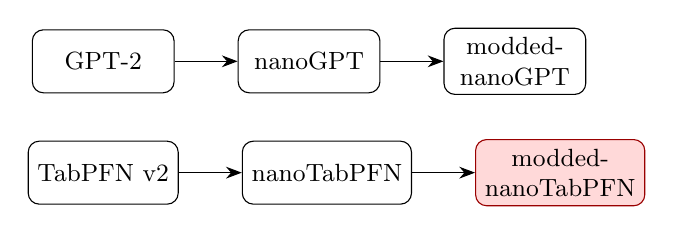
\begin{tikzpicture}[
      node distance=6mm and 8mm,
      box/.style={draw, rounded corners, minimum height=8mm, minimum width=18mm, align=center, font=\small},
      ours/.style={box, fill=red!15, draw=red!60!black},
      arr/.style={-{Stealth[length=2mm]}},
    ]
    \node[box]                  (gpt)  {GPT-2};
    \node[box, right=of gpt]    (nano) {nanoGPT};
    \node[box, right=of nano]   (mod)  {modded-\\nanoGPT};
    \node[box, below=of gpt]    (tab)  {TabPFN v2};
    \node[box, right=of tab]    (ntab) {nanoTabPFN};
    \node[ours, right=of ntab]  (mtab) {modded-\\nanoTabPFN};
    \draw[arr] (gpt)  -- (nano);
    \draw[arr] (nano) -- (mod);
    \draw[arr] (tab)  -- (ntab);
    \draw[arr] (ntab) -- (mtab);
  \end{tikzpicture}
  \caption{Lineage of our work. The language side (top) is established, modded-nanoTabPFN (red) is the contribution of this paper.}
  \label{fig:lineage}
\end{figure}

\section{Related Work}

\paragraph{Tabular Foundation Models.}
Tabular foundation models pretrain a transformer on synthetic datasets and then make predictions on new tasks via in-context learning. 
TabPFN~\citep{hollmann2023tabpfn,hollmann2025tabpfnv2} pioneered this approach, 
followed by TabICL~\citep{qu2025tabicl,qu2026tabiclv2}, TabDPT~\citep{ma2025tabdpt}, and LimiX~\citep{zhang2025limix}.
All these models share an expensive pretraining stage that bottlenecks (todo: what?).
nanoTabPFN~\citep{pfefferle2025nanotabpfn} (todo: if u cite here dont need later) is a minimal, hackable reimplementation of TabPFN v2 designed for educational use and the basis for our competition.
Its short pretraining time came from small-scale data, here we go larger and modify it (todo:update here).

\paragraph{nanoGPT and modded-nanogpt.}
Our format is inspired by community speedrun efforts on language model pretraining.
nanoGPT~\citep{karpathy2023nanogpt} is a minimal, hackable reimplementation of GPT-2 designed for easy prototyping and experimentation.
modded-nanogpt~\citep{moddednanogpt} is a community-driven speedrun built on top of nanoGPT in which contributors compete to reach a fixed validation loss in less wallclock time.
Iterations of the competition have surfaced techniques such as the Muon optimizer~\citep{jordan2024muon}.
We adopt the same speedrun leaderboard format for tabular foundation models.

\paragraph{TabArena. (todo: ?)}
For evaluation we leverage TabArena~\citep{erickson2025tabarena}, a living benchmark for tabular machine learning that curates a representative collection of classification and regression datasets and maintains a public leaderboard.
We use the curated datasets to measure downstream performance of pretrained models, but do not adopt the full benchmark protocol. This lets us inherit the dataset diversity while keeping evaluation fast enough for rapid iteration.

\section{Competition}
\lipsum[1]

\subsection{Rules}
\lipsum[1]

\subsection{Evaluation}
\lipsum[1]

\begin{figure*}[t]
  \centering
  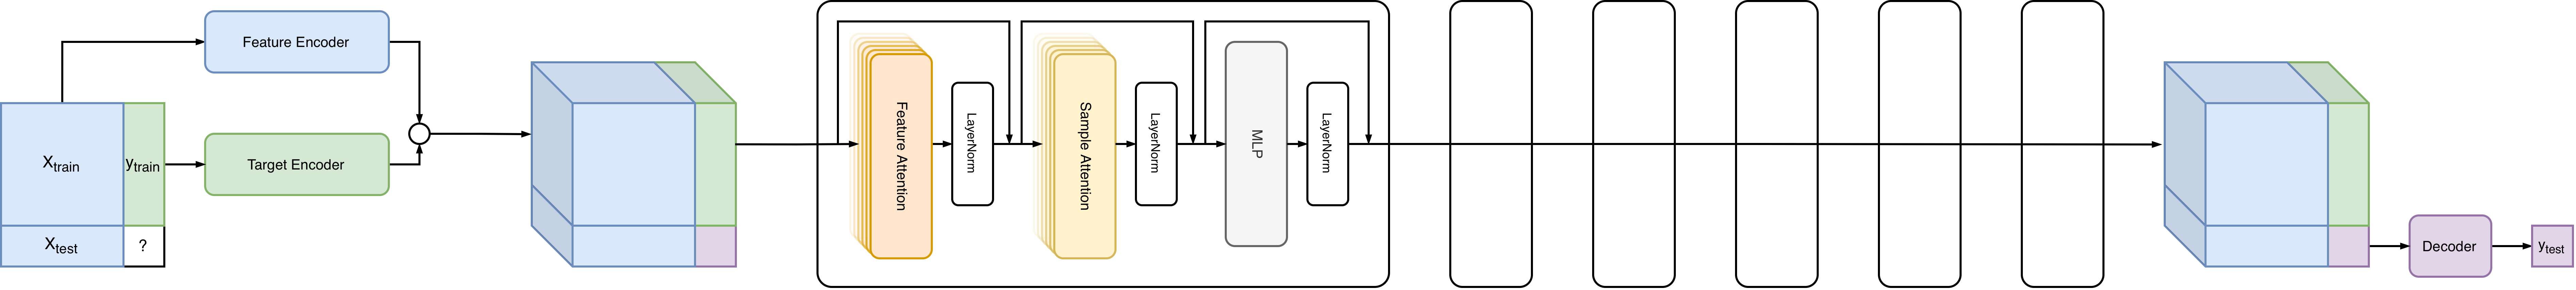
\includegraphics[width=\textwidth]{images/base.png}
  \caption{}
  \label{fig:base}
\end{figure*}

\begin{figure*}[t]
  \centering
  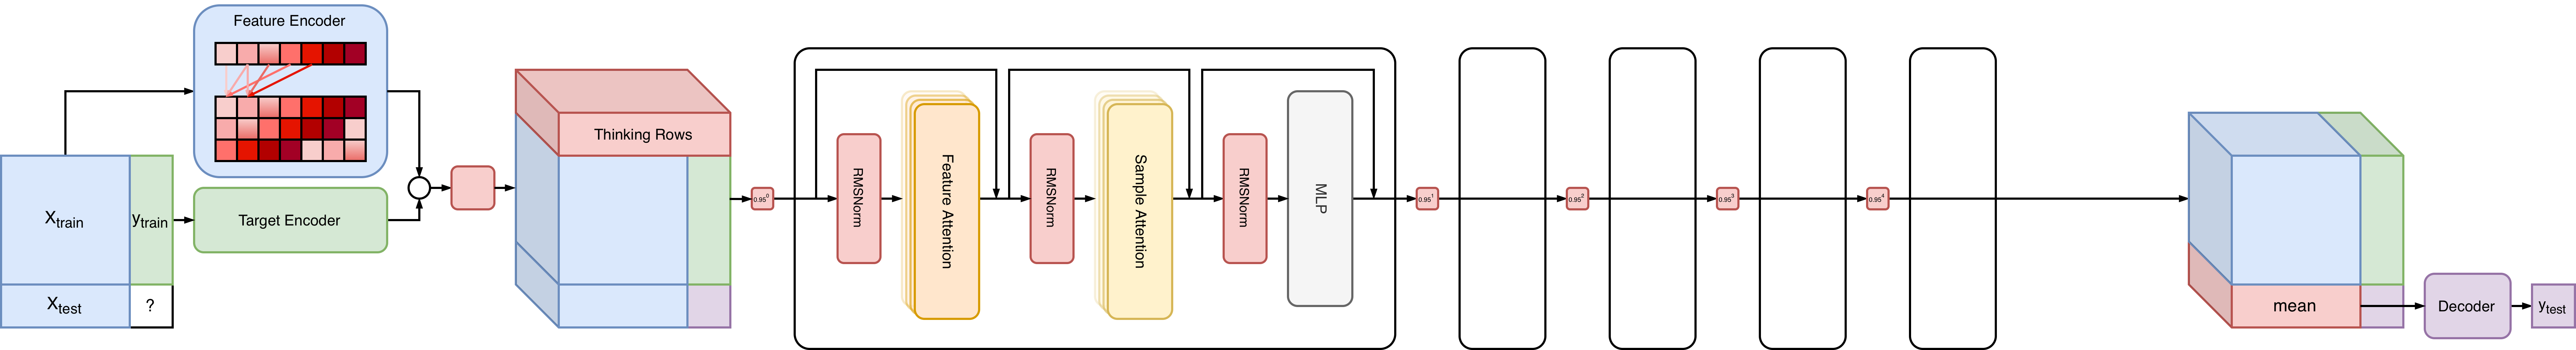
\includegraphics[width=\textwidth]{images/modded.png}
  \caption{}
  \label{fig:modded}
\end{figure*}

\section{Speedrun Results}
\lipsum[1-8]

\begin{figure}[t]
  \centering
  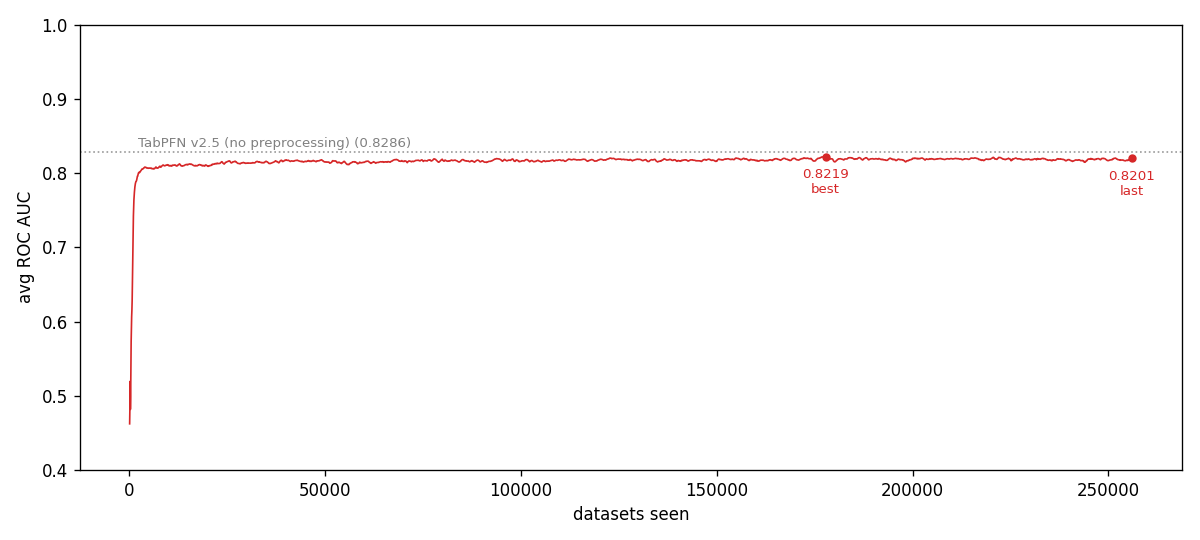
\includegraphics[width=\columnwidth]{images/longrun.png}
  \caption{}
  \label{fig:longrun}
\end{figure}

\section{Conclusion}
\lipsum[2]

\todo[inline]{autoresearch(https://github.com/karpathy/autoresearch) NAS(nerual architecture search) and HPO(hyperparamerter optimisation) connection}
\todo[inline]{LLM usage}

% Acknowledgements should only appear in the accepted version.
\section*{Acknowledgements}
\todo[inline]{maybe carter here}

\section*{Impact Statement}

\bibliography{main}
\bibliographystyle{icml2026}

\newpage
\appendix
\onecolumn
\section{Appendix}

\subsection{Records}
\subsubsection{}

\end{document}
